\subsection{Network analysis}
To get a better understanding of the network traffic behind the malicious application a network analysis was performed.
The process and results of the network analysis are described in this chapter.

\subsubsection{HTTP proxy analysis}
Mitmproxy was used to capture the network traffic to and from the emulated phone.
Mitmproxy ended up showing that the phone made a connection with multiple different IP addresses.
After around 30 minutes of capturing the network traffic it kept connecting and disconnecting with the same 5 IP addresses.
A couple of times an IP address came up that was in a completely different range of IP’s.

In the picture that is shown below there are a total of 8 IP addresses that are captured again and again.
5 out of the 8 IP addresses all started with a 3.
The remaining IP addresses were very different from the 3. range and they were not consistently looping like the others.
In mitmproxy there was not a lot of information that could be analyzed with the software.

\begin{figure}[H]
    \centering
    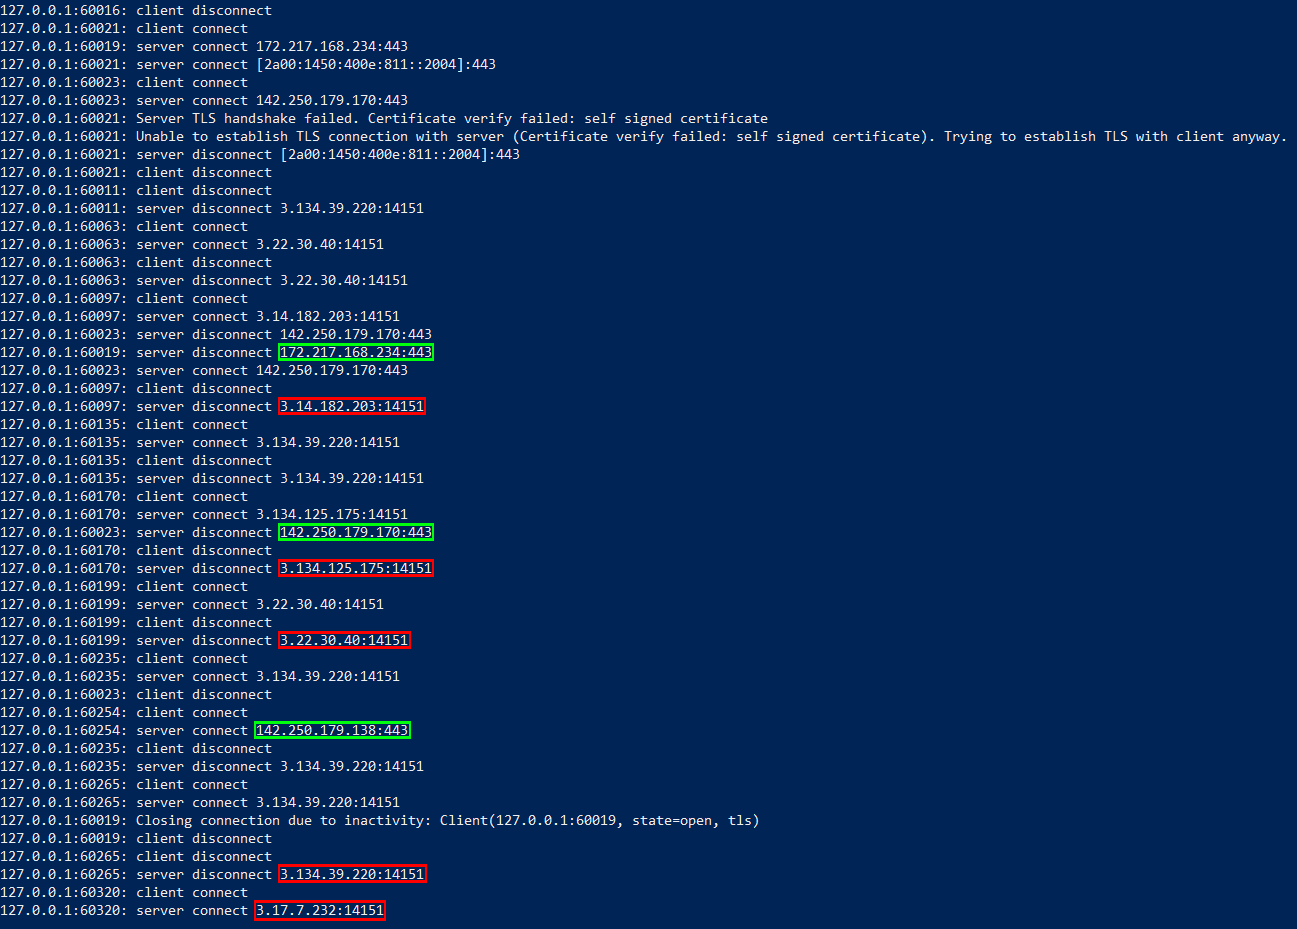
\includegraphics[width=0.85\textwidth]{MitmwebCapture.png}
    \caption{Captured network traffic with mitmproxy}
    \label{jordy-mitmweb}
\end{figure}

\newpage
\subsubsection{Wireshark analysis}
The captured network traffic in mitmproxy indicated that there were multiple connections to different IP addresses.
As described in subchapter 4.3.1 there was 1 range with 5 different IP addresses that kept looping.
The decision was made to focus on these 5 IP addresses since this range of IP’s were described on VirusTotal.
This was done with the following filter in Wireshark:

“(ip.addr == 3.22.30.40 || ip.addr == 3.17.7.232 || ip.addr == 3.134.125.175 || ip.addr == 3.134.39.220 || ip.addr == 3.14.182.203 || ip.src == 3.22.30.40 || ip.src == 3.17.7.232 || ip.src == 3.134.125.175 || ip.src == 3.134.39.220 || ip.src == 3.14.182.203)”.
 
The results of this filter are shown in the picture below.

\begin{figure}[H]
    \centering
    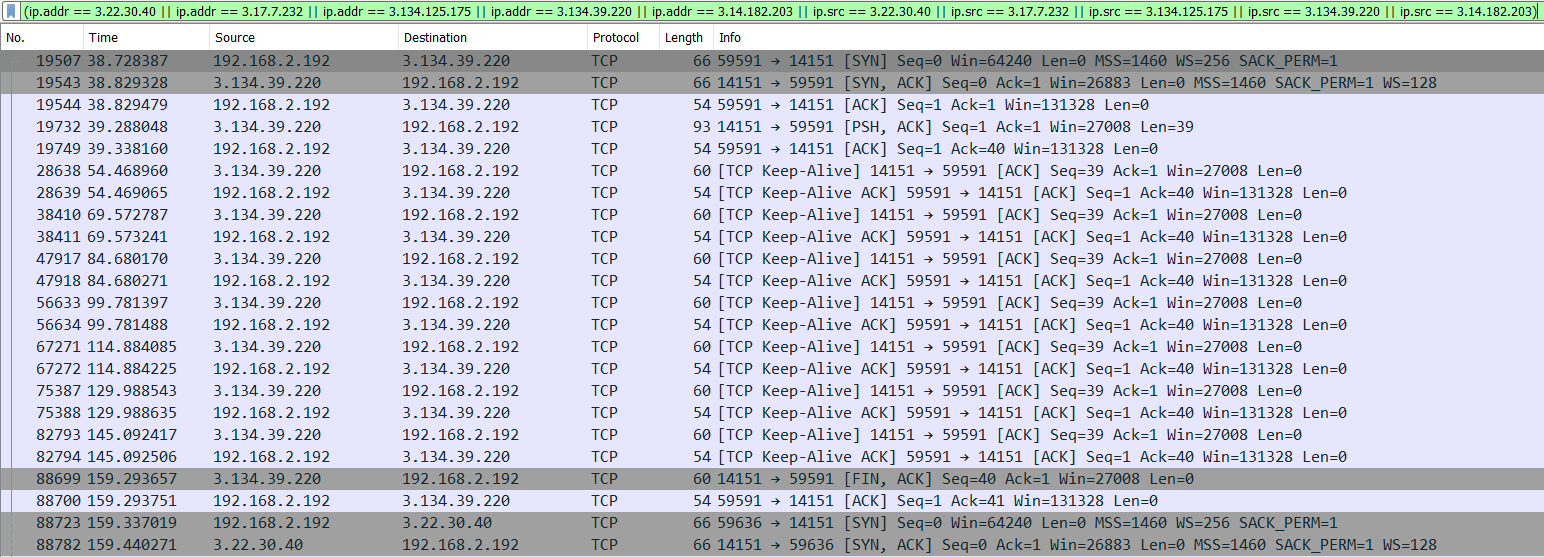
\includegraphics[width=1\textwidth]{WiresharkIPFilter.png}
    \caption{Captured network traffic with Wireshark filter specific IP's}
    \label{jordy-wiresharkfilter}
\end{figure}

Wireshark showed that the connection with different IP addresses all did the exact same thing.
The first grey line showed that the malicious application was asking to make a connection with the IP address.
The second grey line showed that the system on the IP address agreed to make a connection.
 
The first blue described that the two have made a connection.
The second blue line showed that the malicious application sends some data to the IP address.
From here on out it kept the connection alive till the IP address indicated that it wanted to terminate the connection with the third grey line.
From there it showed that both parties agreed to terminate the connection.
When the connection was terminated the application started the exact same process, but with a new IP address.

\newpage
It was not successful to try and determine exactly what data the application send over to the IP address that it made a connection with.
However it is likely that the application sends over information about the phone.

During the Wireshark analysis it was decided that it could be beneficial to look at the DNS traffic.
With the filter “DNS” in Wireshark all the DNS traffic on the laptop was captured.
When the application was installed on the phone one specific DNS stood out.
The specific DNS that stood out was “0.tcp.ngrok.io”.
This DNS was connected with one of the IP addresses that were found with mitmproxy.
The picture below shows the information in Wireshark.

\begin{figure}[H]
    \centering
    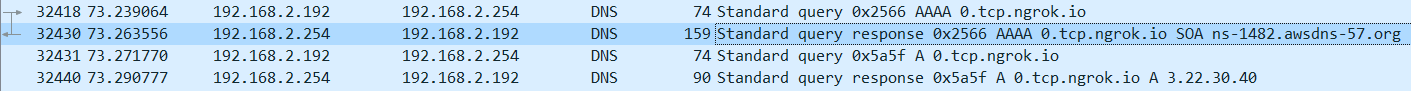
\includegraphics[width=1\textwidth]{WiresharkDNS Capture.png}
    \caption{Captured network traffic with Wireshark filter on DNS}
    \label{jordy-wiresharkDNS}
\end{figure}

It is very likely that behind the DNS “0.tcp.ngrock.io” a command and control server is hosted.

\subsubsection{Reconnaissance}

\href{https://www.shodan.io/host/3.14.182.203}{Shodan.io} was used to find out more about the different IP addresses.
All 5 of the IP addresses in the 3. range were owned by Amazon.
The location of the IP showed up as the city Hilliard in the United States and their server provider was Amazon.
It is likely that the people behind this application rent their servers from Amazon and when they have gotten enough complains or their scam is figured out they change the servers and IP’s that the application uses.
This would explain why the two described IP addresses on VirusTotal have not been seen during the network analysis.

The IP addresses in the 142. and 172. ranges were checked as well with \href{https://www.shodan.io/host/172.217.168.234}{Shodan.io}. It turned out that these IP addresses were owned by Google.
This meant that these IP addresses were not really interesting for the research.

